El sistema implementa perfiles de velocidad trapezoidales con aceleraciones fijas, garantizando comportamiento predecible independientemente de la distancia del movimiento. Las distancias de aceleración y desaceleración permanecen constantes, variando únicamente la longitud de la zona de crucero.

El perfil se compone de las fases mostradas en las Tablas \ref{tab:perfil_horizontal} y \ref{tab:perfil_vertical}. Esta estrategia asegura que las aceleraciones sean idénticas para todos los movimientos, proporcionando comportamiento mecánico consistente.

\begin{table}[H]
\centering
\small
\begin{tabular}{|l|c|c|c|c|}
\hline
\textbf{Fase} & \textbf{Distancia} & \textbf{$v_i$ (m/s)} & \textbf{$v_f$ (m/s)} & \textbf{Aceleración (m/s²)} \\
\hline
1. Arranque & Instant. & 0 & 0.05 & - \\
\hline
2. Acel. suave & 5 mm & 0.05 & 0.10 & 0.05 \\
\hline
3. Acel. fuerte & 7.5 mm & 0.10 & 0.375 & 0.37 \\
\hline
4. Crucero & Variable & 0.375 & 0.375 & 0 \\
\hline
5. Decel. fuerte & 7.5 mm & 0.375 & 0.10 & -0.37 \\
\hline
6. Decel. suave & 5 mm & 0.10 & 0.05 & -0.05 \\
\hline
7. Detención & Instant. & 0.05 & 0 & - \\
\hline
\end{tabular}
\caption{\textit{Fases del perfil trapezoidal de velocidad para movimiento horizontal}}
\label{tab:perfil_horizontal}
\end{table}

\begin{table}[H]
\centering
\small
\begin{tabular}{|l|c|c|c|c|}
\hline
\textbf{Fase} & \textbf{Distancia} & \textbf{$v_i$ (m/s)} & \textbf{$v_f$ (m/s)} & \textbf{Aceleración (m/s²)} \\
\hline
1. Arranque & Instant. & 0 & 0.05 & - \\
\hline
2. Acel. suave & 5 mm & 0.05 & 0.10 & 0.05 \\
\hline
3. Acel. fuerte & 7.5 mm & 0.10 & 0.30 & 0.27 \\
\hline
4. Crucero & Variable & 0.30 & 0.30 & 0 \\
\hline
5. Decel. fuerte & 7.5 mm & 0.30 & 0.10 & -0.27 \\
\hline
6. Decel. suave & 5 mm & 0.10 & 0.05 & -0.05 \\
\hline
7. Detención & Instant. & 0.05 & 0 & - \\
\hline
\end{tabular}
\caption{\textit{Fases del perfil trapezoidal de velocidad para movimiento vertical}}
\label{tab:perfil_vertical}
\end{table}

\begin{figure}[H]
    \centering
    % TODO: Insertar gráfico comparativo mostrando mismo perfil de aceleración para diferentes distancias
    % Mostrar: dos movimientos (25mm vs 250mm) con mismas rampas de accel/decel pero diferente zona crucero
    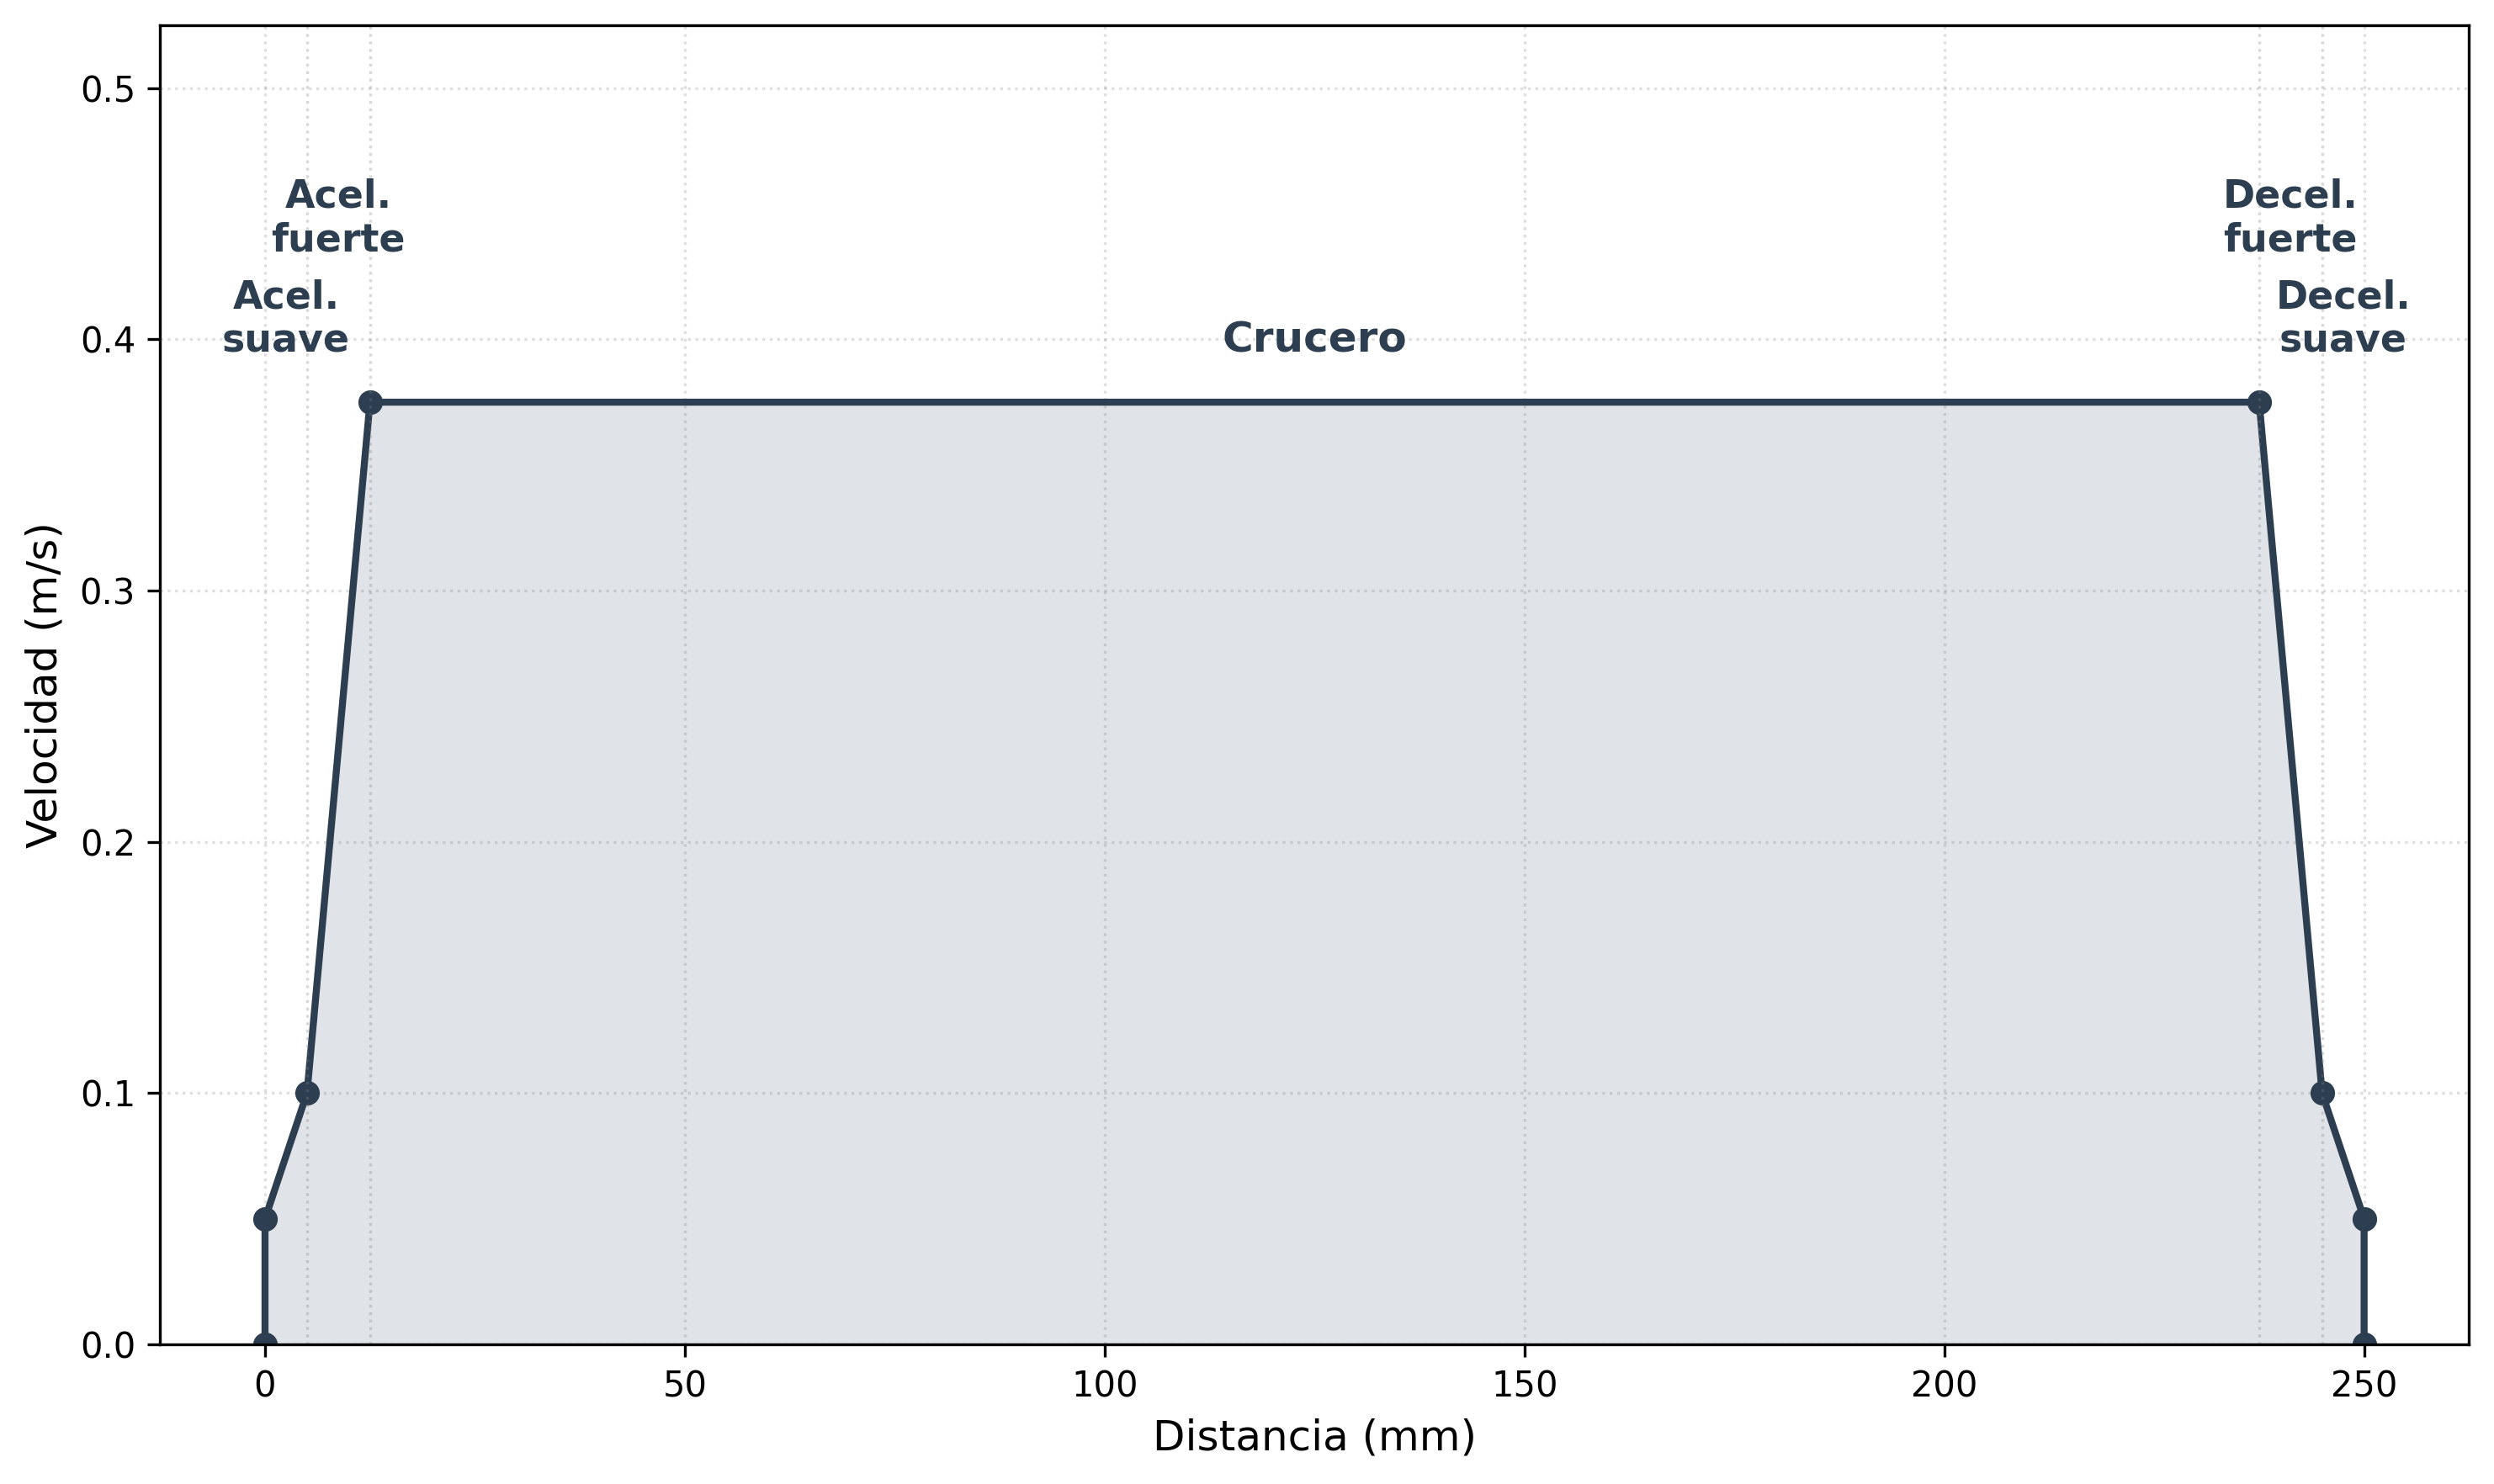
\includegraphics[width=0.7\textwidth]{imagenes/perfil_trapezoidal_velocidad.png}
    \caption{\textit{Perfil trapezoidal con aceleraciones fijas. Las zonas de aceleración y desaceleración mantienen longitud constante (12.5mm cada una), mientras que la zona de crucero se ajusta según la distancia total}}
    \label{fig:perfil_trapezoidal}
\end{figure}

Cuando la distancia total es menor que 25mm, el perfil se convierte en triangular. El sistema mantiene las mismas aceleraciones de la Tabla \ref{tab:perfil_trapezoidal}, pero calcula el punto medio del movimiento donde debe iniciar la desaceleración para alcanzar exactamente la posición final. En este caso, la velocidad máxima alcanzada es menor que la velocidad de crucero nominal, ya que el motor comienza a frenar antes de alcanzarla. 

Para movimientos muy cortos (menos de 3 mm), el sistema reduce la velocidad máxima permitida a 0.10 m/s para mantener precisión en el posicionamiento final, típico en operaciones de ajuste fino.

\begin{figure}[H]
    \centering
    % TODO: Insertar gráfico comparativo: perfil trapezoidal vs triangular
    % Mostrar: movimiento largo con zona crucero vs movimiento corto sin zona crucero (triangular)
    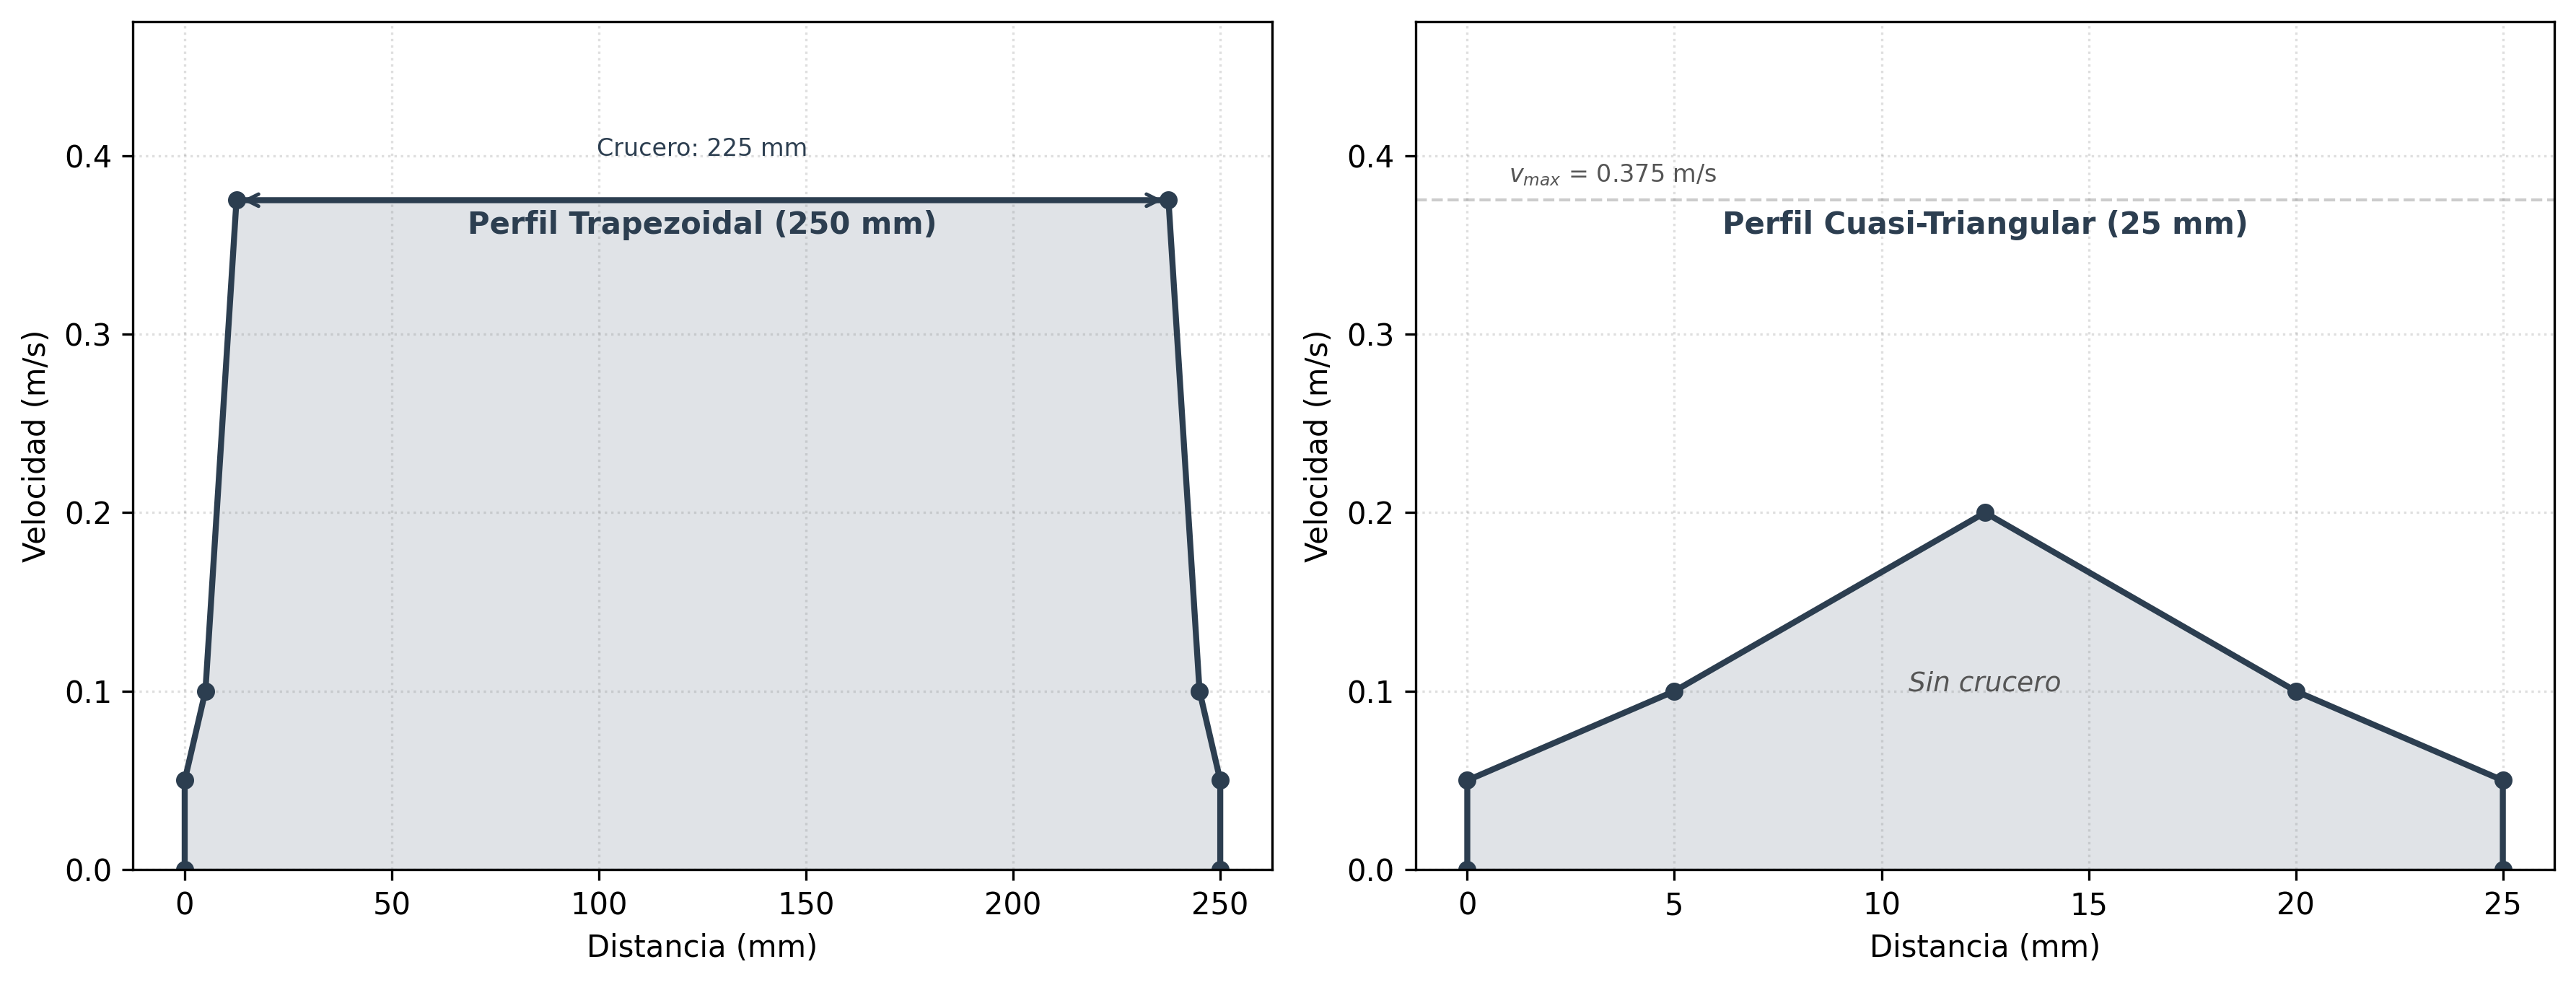
\includegraphics[width=0.7\textwidth]{imagenes/perfil_trapezoidal_triangular.png}
    \caption{\textit{Comparación entre perfil trapezoidal (movimientos largos) y triangular (movimientos cortos). Ambos utilizan las mismas aceleraciones, pero el perfil triangular invierte la aceleración en el punto medio}}
    \label{fig:perfil_comparacion}
\end{figure}

La velocidad instantánea en cada paso se calcula mediante interpolación lineal dentro de cada zona. El firmware ejecuta este cálculo continuamente, actualizando el registro OCR1A del Timer1 que controla la frecuencia de generación de pulsos STEP. La conversión entre velocidad deseada $v$ (en pasos/s) y el valor del registro es:

\begin{equation}
OCR1A = \frac{f_{CPU}}{2 \cdot prescaler \cdot v} - 1 = \frac{1,000,000}{v} - 1
\end{equation}

donde $f_{CPU} = 16$ MHz y prescaler = 8. El sistema soporta velocidades entre 500 pasos/s (inicio/fin de movimientos) y 15,000 pasos/s (crucero máximo). Velocidades superiores causan jitter excesivo y riesgo de pérdida de pasos.

Para movimientos diagonales que involucran ambos ejes simultáneamente, el firmware sincroniza los perfiles mediante escalamiento proporcional de velocidades. El eje con mayor distancia a recorrer (eje dominante) utiliza su velocidad de crucero nominal, mientras que el eje subordinado escala su velocidad proporcionalmente: $v_{sub} = v_{dom} \times (d_{sub}/d_{dom})$. Este escalamiento se aplica a todas las fases del perfil, garantizando que ambos ejes completen el movimiento casi al mismo tiempo y generando trayectorias rectilíneas en el plano XY (Figura \ref{fig:sincronizacion_multieje}).

\begin{figure}[H]
    \centering
    % TODO: Insertar diagrama de sincronización multi-eje
    % Mostrar: dos ejes con diferentes distancias, perfiles escalados, trayectoria rectilínea resultante
    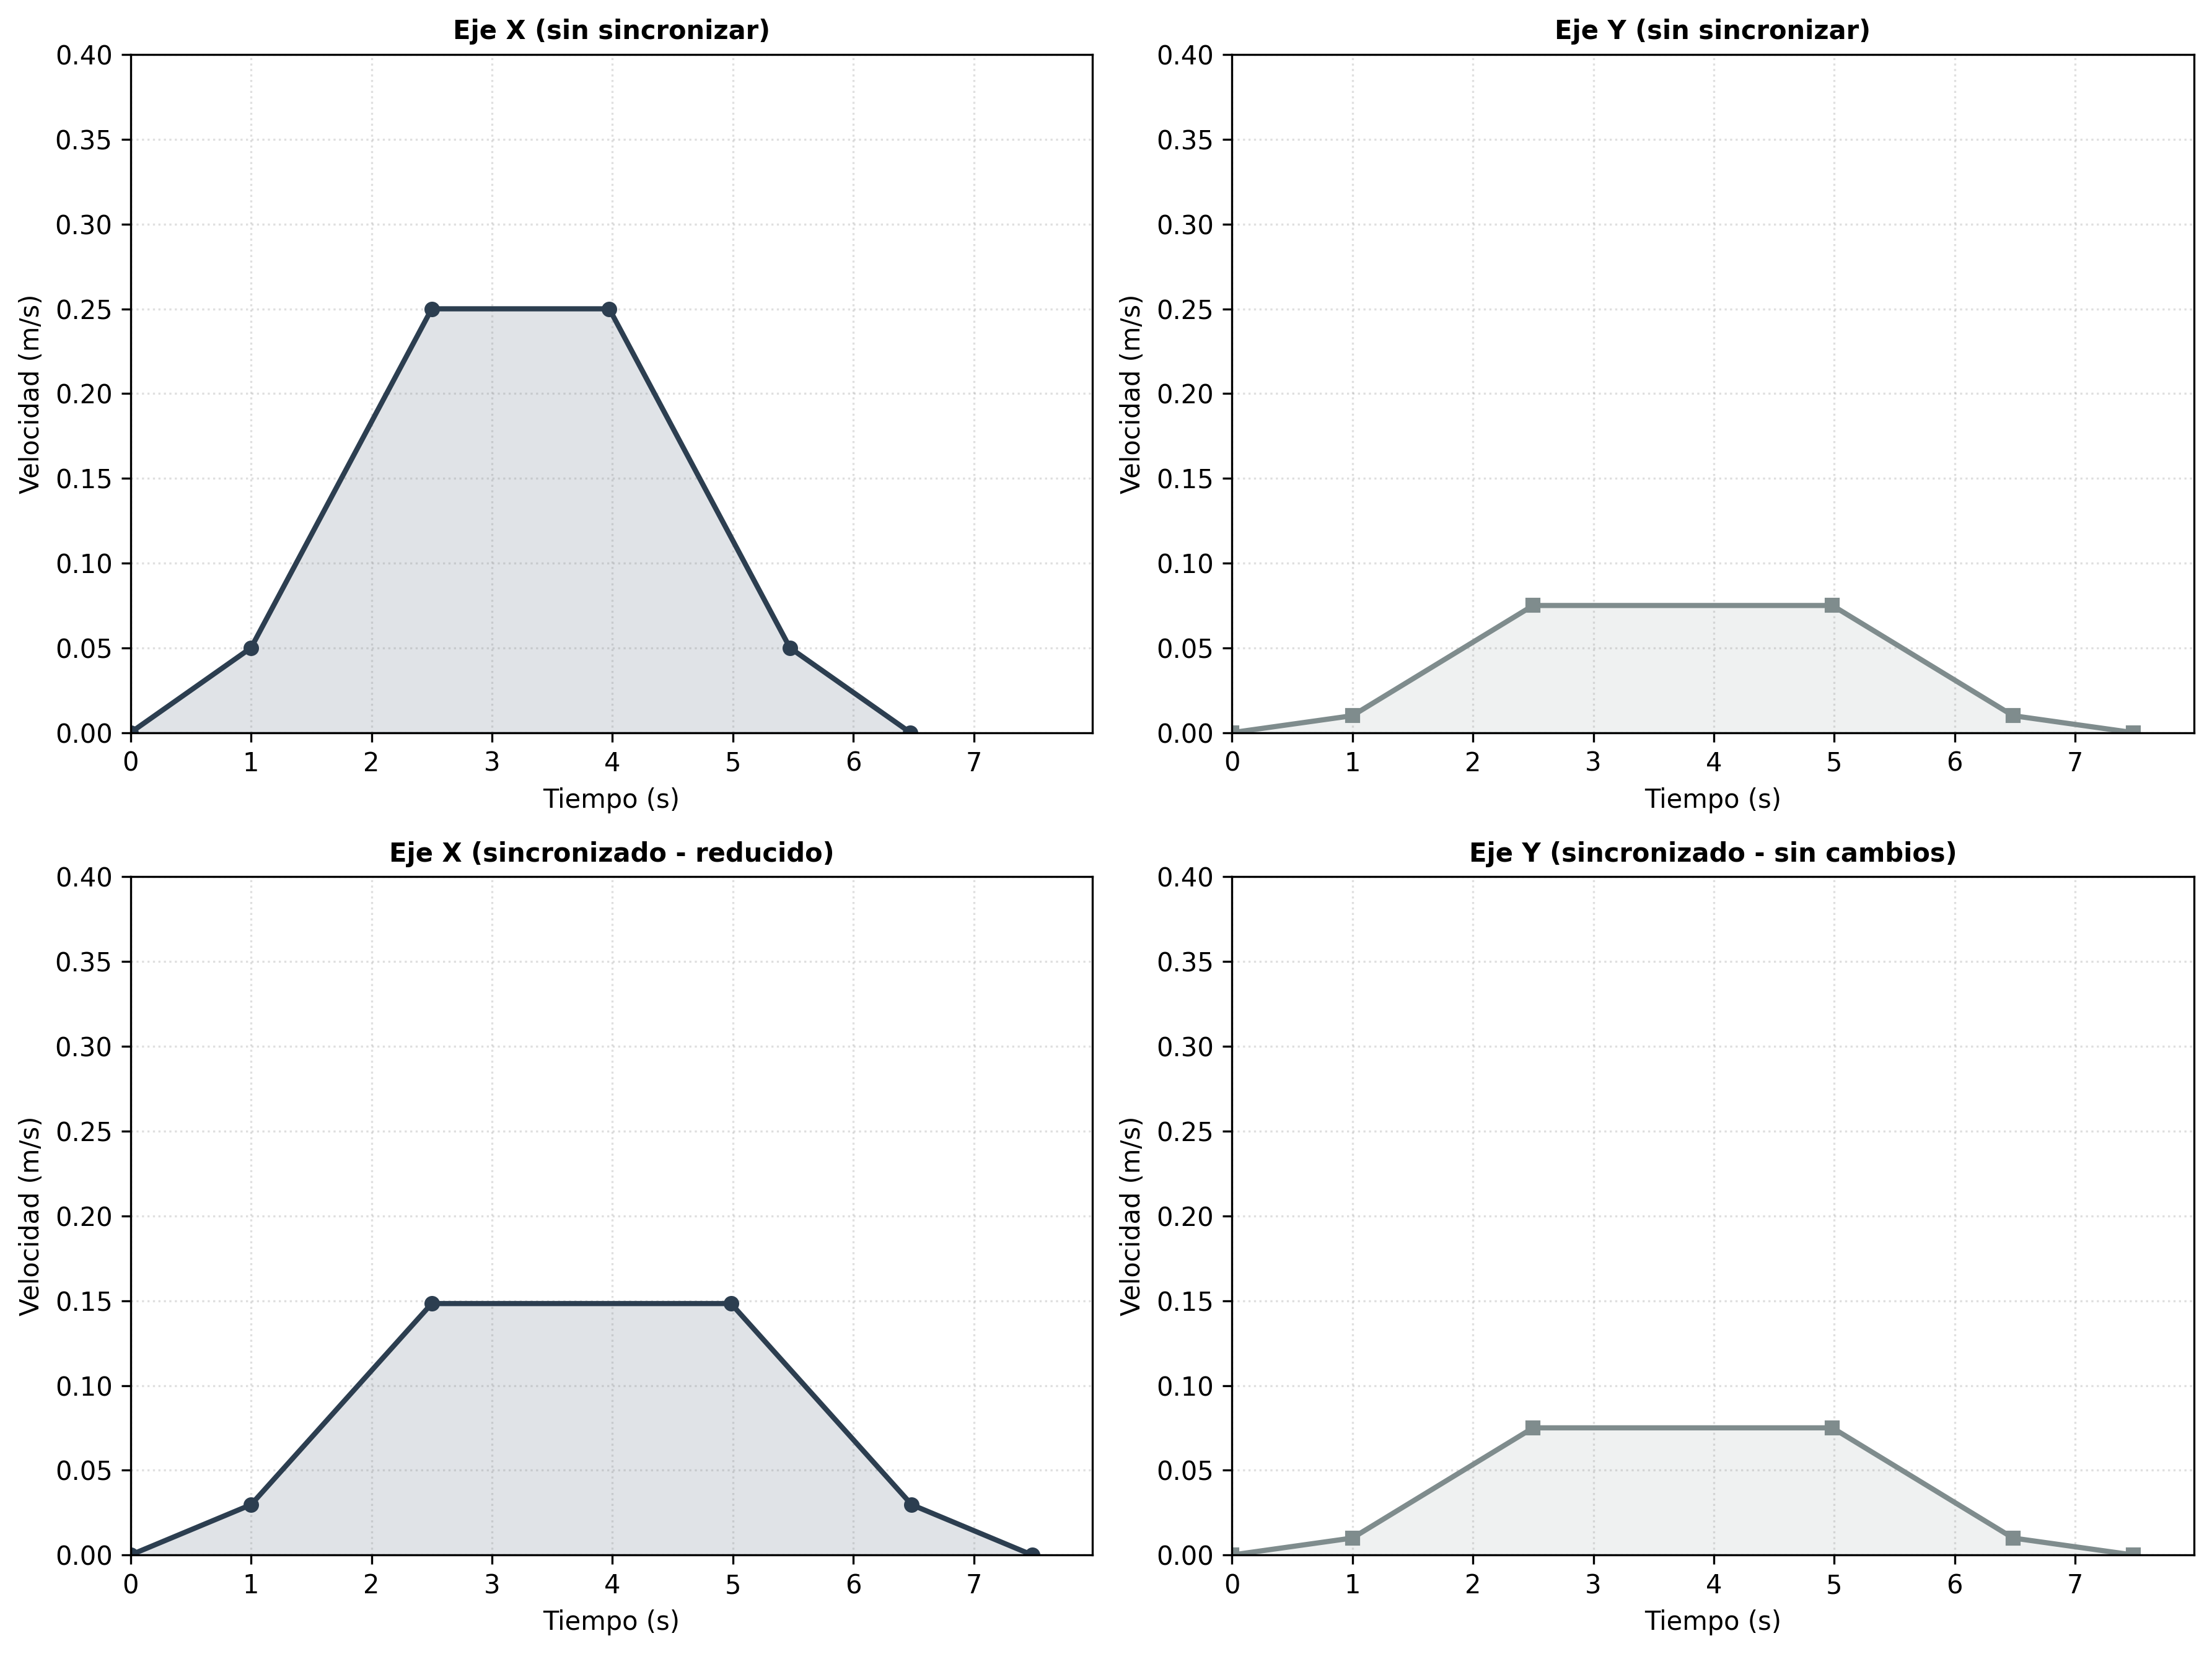
\includegraphics[width=0.7\textwidth]{imagenes/sincronizacion_multieje.png}
    \caption{\textit{Sincronización de perfiles de velocidad para movimientos diagonales mediante escalamiento proporcional}}
    \label{fig:sincronizacion_multieje}
\end{figure}
